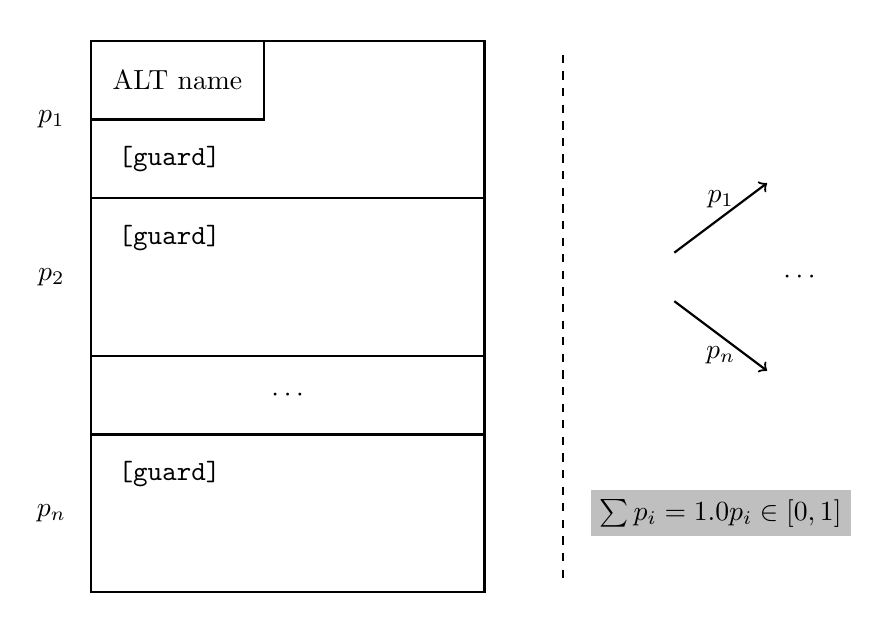
\begin{tikzpicture}[thick]
%%%%%%%%%%%%%%%%%%%%%%%%%%%%%%%%%%%%%%%%%%% HELP LINES
%\draw[help lines] (0,0) grid +(10,10);

%%%%%%%%%%%%%%%%%%%%%%%%%%%%%%%%%%%%%%%%%%% elements
\draw (1,0) rectangle +(5,2);
\node[shape=rectangle, draw=none](p1) at (0.5,6){$p_1$};
\draw (1,2) rectangle +(5,1);
\node[shape=rectangle, draw=none](p2) at (0.5,4){$p_2$};
\draw (1,3) rectangle +(5,2);
\node[shape=rectangle, draw=none](pn) at (0.5,1){$p_n$};
\draw (1,5) rectangle +(5,2);
\node[shape=rectangle, draw=none](ellipsis) at (3.5,2.5){$\cdots$};
\node[circle, draw=none](t1) at (7,7){};
\node[circle, draw=none](t2) at (7,0){};
\node[circle, dashed, minimum size=1cm] (current) at (8,4){};
\node[circle, minimum size=1cm] (a1) at (10,5.5){};
\node[circle, draw=none] (ai) at (10,4){$\cdots$};
\node[circle, minimum size=1cm] (a2) at (10,2.5){};

%%%%% guards and constraints
\node[shape=rectangle, draw=black, minimum height=1cm, minimum width=2.2cm](alt)at(2.1,6.5){ALT name};
\node[shape=rectangle, draw=none](guard1) at (2,5.5) {\texttt{[guard]}};
\node[shape=rectangle, draw=none](guard2) at (2,4.5) {\texttt{[guard]}};
\node[shape=rectangle, draw=none](guard3) at (2,1.5) {\texttt{[guard]}};
\node[shape=rectangle, fill=gray!50, draw=none](constraint) at (9,1) {$\sum p_{i}=1.0$ \\ $p_{i} \in [0,1]$};

%%%%% edges
\draw[dashed] (t1) -- (t2);
\draw[->, thick] (current) -- node[draw=none,above]{$p_1$}(a1);
\draw[->, thick] (current) -- node[draw=none,below]{$p_n$}(a2);
\end{tikzpicture}

